\section{Vorlesung 16}
\subsection{Mäuse problem}
\begin{flushleft}
	4 Mäuse = 4 Masse punkte 
gleichschnell, gleich förmige Bewegung zu jedem Punkt bewegt sich $m_i$ auf $m_{i+1}$ zu.
Bahnkkurve der Mäuse ? Z.B für $m_0$\\
$y(t)= \begin{pmatrix}
x(t)\\
y(t)
\end{pmatrix}$
Sei $M_0$ zu Punkt t m Punkt $p_0(x(t),y(t))$\\
 $\Rightarrow m_1$ ist im Punkt $p_1 (-y(t),x(t))$\\
$\underset{\underset{\text{Tangentenrichtung an Bahnkurve (entspricht) Ableitung} }{\uparrow}}{Richtungsvektor}$  : $p_1 - p_0 = \begin{pmatrix}
 									-y(t) - x(t)\\
									 x(t)-y(t)
								\end{pmatrix}$\\
								
								$Y' (t)=\begin{pmatrix}
									x'(t)\\
									y'(t)
								\end{pmatrix}=C . \begin{pmatrix}
								-y(t) - x(t)\\
								x(t)-y(t)
								\end{pmatrix}$
								wählen C=1\\ 
 \textbf{Lösung} \\
ges: sind 2 linear unabh. \\
lösungen: $Y_1(t), Y_2(t)$.	\\
$\Rightarrow $ allg. Lösung: $Y(t) = C_1 Y_1(t)+C_2 Y_2(t) \qquad, C_1,C_2\in \mathbb{R}$\\
Eigenwete:\\
$det(A-\lambda E_2)= \left| \begin{matrix}
	-1-  \lambda \quad &-1\\
	1			 \quad &-1-\lambda
\end{matrix}\right|$\\
$=(-1-\lambda)^2 +1 =0$\\
$=\lambda^2+2\lambda +2=0$\\
$\overset{pq.formel}{\Rightarrow} \lambda_1,2=-1\pm i$\\
Es existert keine rellen Eigenvektoren.\\
\textbf{Trick}\\
Erweiterung des Zahlbereich: $\mathbb{R} \leadsto \mathbb{C}$\\
Eigenraum zu $\lambda_1 = -1+i:$\\
$\begin{pmatrix}
	-1-(-1+i)   &-1\\
	1 			&-1-c-1+i
\end{pmatrix}$$\begin{pmatrix}
x_1\\
x_2
\end{pmatrix}$= $\begin{pmatrix}
0\\
0
\end{pmatrix}$\\
$\begin{pmatrix}
-i &-1\\
1  &-i
\end{pmatrix}$
$\begin{pmatrix}
x_1\\
x_2
\end{pmatrix} $ $=\begin{pmatrix}
	0\\
	0
\end{pmatrix}$\\
$-ix_1-x_2=0$\\
$x_2=-ix_1$\\
$ \Rightarrow Eig_A (\lambda_1)=span(\{ \begin{pmatrix}
		i\\
		1
	\end{pmatrix} \})$	\\
für $\lambda_2=\overline{\lambda_1}	$	ist\\
$Eig_A(\lambda_2)=span(\{ \underbrace{\begin{pmatrix}
-1\\
1
\end{pmatrix}}_{:= \overline{V}}  \})	$	\\
$\Rightarrow $Allg. komplexe Lösung:\\
$Y_\mathbb{C}(t)=C_1e^{\overline{\lambda_1}(t)}	\overline{V},C_1,C_2 \in \mathbb{C}	$\\
$Re(e^{\lambda_1 t }V  ) $ und $Im(e^{\lambda t}V)$	\\
sind l.u reelle Lösungen
$e^{\lambda_1 t}V= e^{(-1+i)t}(\begin{pmatrix}
	0\\
	1
\end{pmatrix}+i\begin{pmatrix}
	1\\
	0
\end{pmatrix})$\\
$e^{-t}(\cos t+ i \sin t)(\begin{pmatrix}
0\\
1
\end{pmatrix} +i\begin{pmatrix}
1\\
0
\end{pmatrix})$
$e^{\lambda_1 t}V=e^-t (\cos \begin{pmatrix}
0\\
1
\end{pmatrix}+i^2 \sin t \begin{pmatrix}
1\\
0
\end{pmatrix}+i \cos t \begin{pmatrix}
1\\
0
\end{pmatrix})                              $\\
$=\underbrace{e^{-t}\begin{pmatrix}
-\sin t\\
\cos t
\end{pmatrix}}_{Reelleteil}+\underbrace{i e^{-t}\begin{pmatrix}
\cos t\\
\sin t
\end{pmatrix}}_{Imag.teil}$\\
$\Rightarrow$ Allg. reelle Lösung\\
$Y(t)= C_1 e^{-t}\begin{pmatrix}
\cos t\\
\sin t
\text { für } \end{pmatrix}= \underbrace{e^{+t}}_{ \underset{ \text{ für } t \rightarrow \infty}{\rightarrow 0} } \underbrace{\begin{pmatrix}
	\cos t   &-\sin t\\
	\sin t   &\cos t
\end{pmatrix}}_{Rotationsmatrix} \begin{pmatrix}
C_1\\
C_2
\end{pmatrix}$\\
$C_1 , C_2\in \mathbb{R}$\\
Spezielle lösung für $m_0$: Startpunkt $ Y_s(0)=	\begin{pmatrix}
	1\\
	1
\end{pmatrix}$	\\
$Y_s(0)= C_1 e^{-t}\begin{pmatrix}
\cos t\\
\sin t
\text { für } \end{pmatrix}= e^{-0} \begin{pmatrix}
	\cos 0   &-\sin 0\\
	\sin 0   &\cos 0
	\end{pmatrix}\begin{pmatrix}
C_1\\
C_2
\end{pmatrix}$	\\
$\Rightarrow Bahn Kurve von M_0: Y_s(t)e^{-t}	\begin{pmatrix}
-\sin t+\cos t\\
\cos t+ \sin t
\end{pmatrix}$			
 Lineare Dgl. in n-ter Ordnung mit konst. Koeffizienten.
\end{flushleft}
 \begin{example}
 	$y"+5y'+6y=0$ harmon. Oszillator\\
 	Allg. n-ter Ordnung \\
 	$y^(n)*a_1y^{(n1)}+\dots+ a_{n-1}y'+a_n y=0$\\
 	im ein System 1. Ordnung umschreiben:\\
\begin{align*}
	&y_1' := y' =y_2   				\quad & \overset{Ableitung}{\curvearrowright} \qquad  &y_1'=y'=y_2 \\
	&y_2:= y' 	  	  		 		 &	\quad		    						   &y_2'=y"=y_3   \\
 	&\vdots  		  		 		 & \quad    									   &\vdots      \\
 	&	y_n:= y^{(n-1)}				 & 	\quad				 		  &y^{(n)}=-a_1y_n-a_2y_{n-1}-\dots -a_n y_1\\
 	&\text{	für Das Beispiel:} 	  	 &	\quad		&\\
&y_1:= y             			 	\quad&\rightarrow \qquad 												&y_1'=y_2\\
&y_2:=y' 					        & \quad								&y_2'= -5y_2-6y_1
\end{align*}
Dgl. System:\\
$\begin{pmatrix}
y_1'\\
y_2'
\end{pmatrix}= \begin{pmatrix}
0   & 1\\
-6  &-5
\end{pmatrix}\begin{pmatrix}
y_1\\
y_2
\end{pmatrix}$\\
$\left| \begin{matrix}
	-1-  \lambda \quad &\quad-1\\
	1			 \quad &-1-\lambda
\end{matrix}\right| \begin{matrix}
					&= (-\lambda (-5-\lambda))\\
					&=\lambda^2 +5 \lambda +6=0
						\end{matrix}$\\
						$\lambda_1 =-3, \lambda_2=-2$\\
			$\text{Eigenräume:} Eig_a(-3)=span(\{ \begin{pmatrix} 1 \\ 
			-3 \end{pmatrix} \})$
		$\Rightarrow $ allg. Lösung:\\
			$\begin{pmatrix}
					y_1(x)\\
					y_2(x)
			\end{pmatrix}= C_1e^{-3x}	\begin{pmatrix}
			1\\
			-3
		\end{pmatrix}+C_2e^{-2x}\begin{pmatrix}
1\\
-2
	\end{pmatrix} \quad , \quad C_1,C_2\in \mathbb{R}$\\
	Lösung der ursprüngl. Dgl. in 1.Zeile\\
$y(x) = C_1^{-3x}+C_2 e^{-2x} \quad , c_2,C_2 \in \mathbb{R}$\\
$x  \to \infty  $ Stark gedämpfter Oszillator\\
Beobactung für $y"+ay'+by=0$\\
EW-Gleichung \\
$\lambda^2 +a\lambda +b=0$\\
1.) Nullstellen $\lambda_1,\lambda_2\in \mathbb{R}, \lambda_1\neq \lambda_2$\\
$y(x)=C_1e^{\lambda_1 x}+C_2e^{\lambda_2}$\\
$\lambda_{1,2} =-\frac{a}{2}\pm \sqrt{\frac{a^2}{4}-b}$\\
$\lambda_1  \neq \lambda_2 und in \mathbb{R} \frac{a^2}{4}-b >0$\\
2.) Fall : $\frac{a^2}{4}-b=0 \Rightarrow \lambda_1 =\lambda_2=- \frac{a}{2}$\\
Eigenraum gat nur Dim. 1.\\
$y(x)=C_1e^{\lambda_1 x}+ C_2 x. e^{\lambda_1 x}$    $C_1,C_2 \in \mathbb{R}$\\
(skizze! fehlt!)\\
3.) Fall: $\frac{a^2}{4}-b<0$\\
$ \Rightarrow paar Konj. komplexer EW:$\\
$\lambda_{1,2}=\alpha +i\beta (\alpha=- \frac{a}{2}<0)$\\
allg. Lösung:
$y(x)= C_1 e^{\alpha x} \cos (\beta x) +C_2 e^{\alpha x} \sin (\beta x)$\\
Eigentlich ist die welt nicht linear, warum sind linear. system interssant?\\
$y'(t)=F`(Y_{(t)} ) \neq AY$\\
Ruhelagen? $Y'(t)= 0 $ d.h. $ F(Y)=0$\\
sei   $ y_0(t)=y_0 $ konst. eine Ruhelage Tayloretwicklung (linearisierung)\\
$ F(y) \approx F(y_0)+F'(y_0)(y-y_0)$\\
$y(t)-y_0)'\approx F'(y_0)(y_{(t)}-y_0) \qquad (F(y_0)=0)$
 \end{example}
 
\begin{example}[Wettermodell (Edward Lorenz)]

	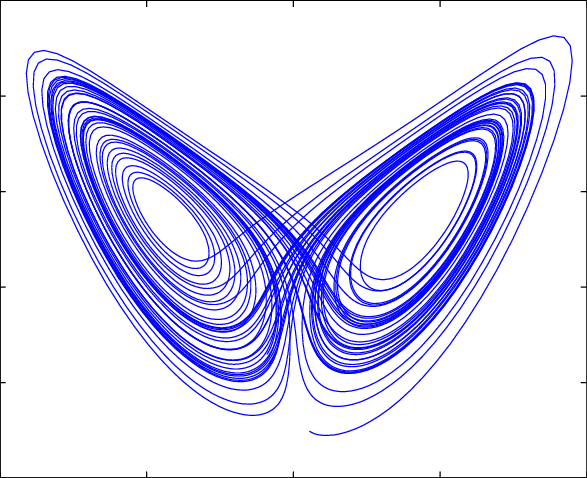
\includegraphics[width=6cm, height=6cm]{images/wettermodell.png}
	


	$x'=-0x+0y$\\
	$y'=-xy+rx-x$\\
	$z'=xy-by$\\
\href{ https://en.wikipedia.org/wiki/Lorenz_system }{Lorenz System Wikipedia}


\end{example}
